\chapter{Validation (part 3): common mistakes and FAQ}\label{ch-11}

The last part on validation collects practical advice on the use of
cross-validation, the \textbf{most frequent mistakes} (especially in
projects) and some examples of model selection, partly taken from the
slides of Andrew W. Moore (CMU).

\section{Stopping training}\label{arresto-delladdestramento}

\subsection{Do not fix an arbitrary number of
epochs}\label{non-fissare-un-numero-arbitrario-di-epoche}

\begin{boxwarning}{Frequent mistake}

Avoid stopping the training of a network after a \textbf{fixed and
arbitrary number of epochs}.

\end{boxwarning}

Why:

\begin{itemize}
\tightlist
\item
  if it is small, one may stop \textbf{too early} (underfitting, or
  favouring high learning rates that require fewer epochs);
\item
  if it is large, one may stop \textbf{too late} (overfitting or wasted
  time);
\item
  the same value cannot be right for all configurations and all
  iterations of a K-fold CV;
\item
  and which number should be used in the final retraining?
\end{itemize}

Even \textbf{selecting the number of epochs via model selection} is not
the best practice: it is better than a fixed number but still imprecise
(because of the problems with K-fold CV and because better criteria
exist). The solutions that work well with a \textbf{well-regularised}
system are those seen in
\href{08\%20-\%20Reti\%20neurali\%20(parte\%202)\%20-\%20addestramento\%20in\%20pratica}{08
- Neural networks (part 2) - training in practice}: look at the
convergence of training (threshold on the error decrease or on the
gradient), or \textbf{early stopping} if one can/wants to use a
validation set.

\subsection{Early stopping}\label{early-stopping}

\begin{boxwarning}{Early stopping and model selection}

The early stopping (ES) criterion is \textbf{part of model selection}
(it must not be applied on the TS): in principle it requires a
\textbf{VL set every time} the model is trained.

\end{boxwarning}

It is delicate: it uses part of the data only to decide when to stop,
without giving a concrete hyperparameter value, and it can become
complex inside a CV. The problem: how to choose the stopping point for
the \textbf{final retraining}, if each fold of the CV has a different
stopping point?

\begin{itemize}
\tightlist
\item
  One could consider the number of epochs as a hyperparameter and take
  the \textbf{mean} over the folds. But changing the amount of data in
  the retraining can change the optimal stopping point (for example
  with more data per epoch, and hence more updates per epoch in
  on-line mode, fewer epochs are needed): one risks under- or
  over-training.
\item
  \textbf{Much better}: take the \textbf{mean training error} at the
  best validation point and use it as a threshold in the retraining,
  to reach the same level of fitting (avoiding under-training effects).
\item
  Otherwise a VL set is needed every time: for example CV with ES
  active in each validation fold (together with the other
  hyperparameters); once the best hyperparameters are found, retrain on
  the recomposed dataset still using part of the data as VL for ES.
\end{itemize}

It is a choice: use ES or rely on \textbf{regularised models} with
standard stopping criteria (e.g.\ no improvement on training). In any
case regularisation helps avoid heavy over-training and reduces the
dependence on ES.

\section{Random initialisation and model
selection}\label{inizializzazione-casuale-e-model-selection}

Different weight initialisations lead to \textbf{different models}. How
to choose the final one (a choice that must be reported in the
report)?

\begin{itemize}
\tightlist
\item
  The \textbf{mean and variance} of the error/accuracy over the
  different trials are computed: a random case will fall within that
  interval, so the risk is under control, unless the variance is high
  (which is in any case a negative signal, see the lecture on bias and
  variance).
\item
  \textbf{All} the models can be used, with an \textbf{ensemble}
  (average of the outputs or vote).
\item
  If \textbf{one} is chosen, that is a \textbf{model selection} and a
  VL set is needed: the \textbf{best} (minimum error on VL), the
  \textbf{median} (a more cautious choice), or a \textbf{random} one (in
  this case no VL set is needed).
\item
  ``Unlucky'' cases can also be discarded by looking only at the
  training error.
\end{itemize}

\section{Sequential hyperparameter
selection}\label{selezione-sequenziale-degli-iperparametri}

\begin{boxwarning}{Frequent mistake}

Selecting the hyperparameters \textbf{one at a time}, sequentially,
introduces an \textbf{order-related bias}. Example: choosing the best
\(\eta\) with 10 units and then using it also with 100 units.

\end{boxwarning}

The correct procedure:

\begin{enumerate}
\def\labelenumi{\arabic{enumi}.}
\tightlist
\item
  initial trials to determine the right \textbf{ranges} (for example by
  looking at the stability of training) and the most
  \textbf{influential} hyperparameters (for example by looking at the
  variance of the results);
\item
  search on a \textbf{grid with all combinations} of the
  hyperparameters (more hyperparameters and values → larger table);
\item
  possibly \textbf{nested} grids, from coarse to fine, on smaller and
  smaller intervals, but considering \textbf{all the significant
  hyperparameters together}, so as to take cross-effects into account.
\end{enumerate}

But: reason, select the relevant aspects, do not rely only on
systematic, expensive automatic approaches. The time constraints of the
project should push towards simple and fast schemes, but correct and
reasonable ones.

\section{What to do after selection and
assessment?}\label{cosa-fare-dopo-selezione-e-valutazione}

\begin{boxquestion}{Can I redesign the model based on the test result?}

No: it is not the correct way and it is not really advantageous (unless
new data are available for a new test set). By repeating this procedure
on the same data one can obtain any result one wants, adapting the
model to that dataset: the model can become perfect on it and not in
future use, and \textbf{one is no longer estimating the risk}.

\emph{The predictor must not be tuned (by hand or automatically) on
the basis of the test error, because we could not do so on future
examples.} In competitions the blind test prevents exactly this. The
evaluation on an internal test is nonetheless useful to \textbf{check
one's own approach}.

\end{boxquestion}

The temptation to decide based on the results is a ``psychological''
problem, external to ML methods. At least be aware of it, or better:

\begin{itemize}
\tightlist
\item
  to build a \textbf{good model} one must do a \textbf{good model
  selection};
\item
  to estimate the \textbf{real performance} one must do a
  \textbf{rigorous} estimate on the test.
\end{itemize}

\section{Cross-validation can
overfit}\label{la-cross-validation-puuxf2-andare-in-overfitting}

Can intensive use of cross-validation lead to overfitting?
\textbf{Yes}, and it retains the problems already seen. Example with
feature selection:

\begin{itemize}
\tightlist
\item
  dataset with 20--30 records and 1000 attributes;
\item
  1000 linear regression models are tried, each with a single
  attribute;
\item
  the best of the 1000 looks good (on the validation set)\ldots{} but it
  would have looked good even with a \textbf{purely random} output!
\end{itemize}

Or (wrong usage): approximating a random target, with a K-fold CV for
the test one finds an error of 3\% instead of the true 50\%, after
choosing the features by best correlation with the targets.
\textbf{Why?} The selection was made on \textbf{all} the examples.

What to do? Keep samples aside \textbf{before} selecting:

\begin{itemize}
\tightlist
\item
  keep an \textbf{additional test set} before any model selection and
  check that the best model also performs well on it;
\item
  for model selection with CV: use ``\textbf{CV + test}'' or
  \textbf{double CV} (redoing the selection for each fold);
\item
  for assessment with CV: do the \textbf{feature selection inside each
  fold}. This gives the correct estimate, about 50\% for the random
  task.
\end{itemize}

\section{Which cross-validation?}\label{quale-cross-validation}

{\def\LTcaptype{none} % do not increment counter
\begin{longtable}[]{@{}
  >{\raggedright\arraybackslash}p{(\linewidth - 4\tabcolsep) * \real{0.3333}}
  >{\raggedright\arraybackslash}p{(\linewidth - 4\tabcolsep) * \real{0.3333}}
  >{\raggedright\arraybackslash}p{(\linewidth - 4\tabcolsep) * \real{0.3333}}@{}}
\toprule\noalign{}
\begin{minipage}[b]{\linewidth}\raggedright
\end{minipage} & \begin{minipage}[b]{\linewidth}\raggedright
Disadvantages
\end{minipage} & \begin{minipage}[b]{\linewidth}\raggedright
Advantages
\end{minipage} \\
\midrule\noalign{}
\endhead
\bottomrule\noalign{}
\endlastfoot
\textbf{Test set (hold-out)} & variance: unreliable estimate of future
performance (luck/bad luck) & cheap \\
\textbf{Leave-one-out} & expensive; has strange behaviours & does not
waste data \\
\textbf{10-fold} & wastes 10\% of the data; 10 times more expensive
than the test set & wastes only 10\%; only 10 times more expensive
instead of \(R\) times \\
\textbf{3-fold} & wastes more data than 10-fold; more expensive than
the test set & slightly better than the test set \\
\textbf{R-fold} (\(R = l\)) & identical to leave-one-out & \\
\end{longtable}
}

\section{Examples of model selection}\label{esempi-di-model-selection}

\subsection{Example 1: different models}\label{esempio-1-modelli-diversi}

\begin{figure}[htbp]
\centering
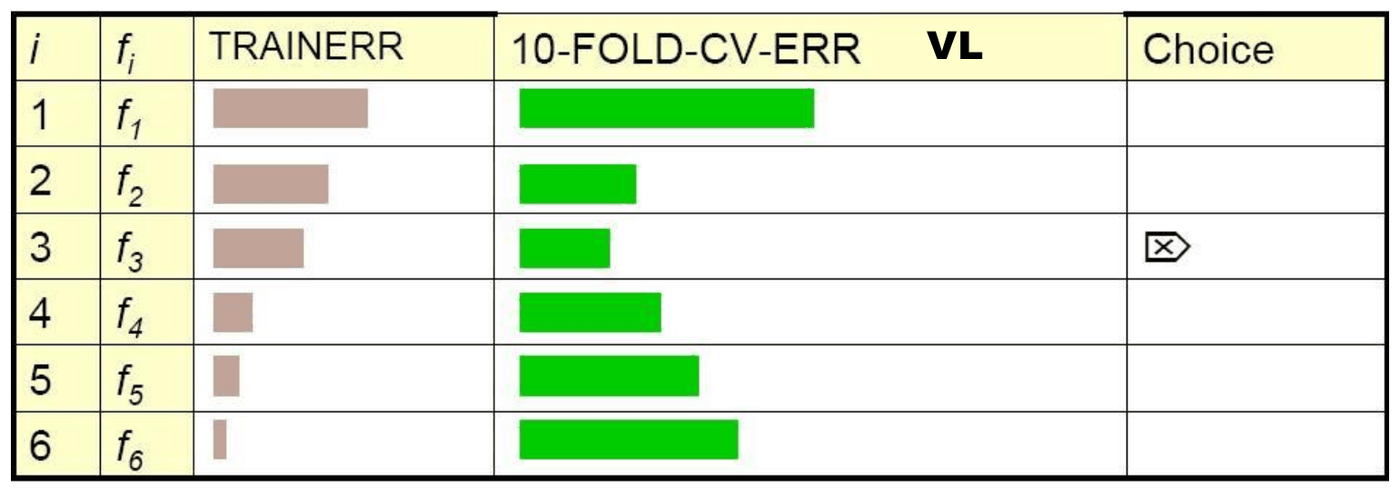
\includegraphics[width=0.86\linewidth,height=0.42\textheight,keepaspectratio]{images/11-val3_es-modelli.png}
\caption{Choice among six classes of models with 10-fold CV.}
\end{figure}

The class of models with the \textbf{best CV score} is chosen, it is
retrained on all the data, and that is the predictive model to use. The
choice is made looking \textbf{only at the validation error},
\textbf{not} at the training error (nor at an average of the two).

\subsection{Example 2: number of hidden
units}\label{esempio-2-numero-di-unituxe0-nascoste}

\begin{figure}[htbp]
\centering
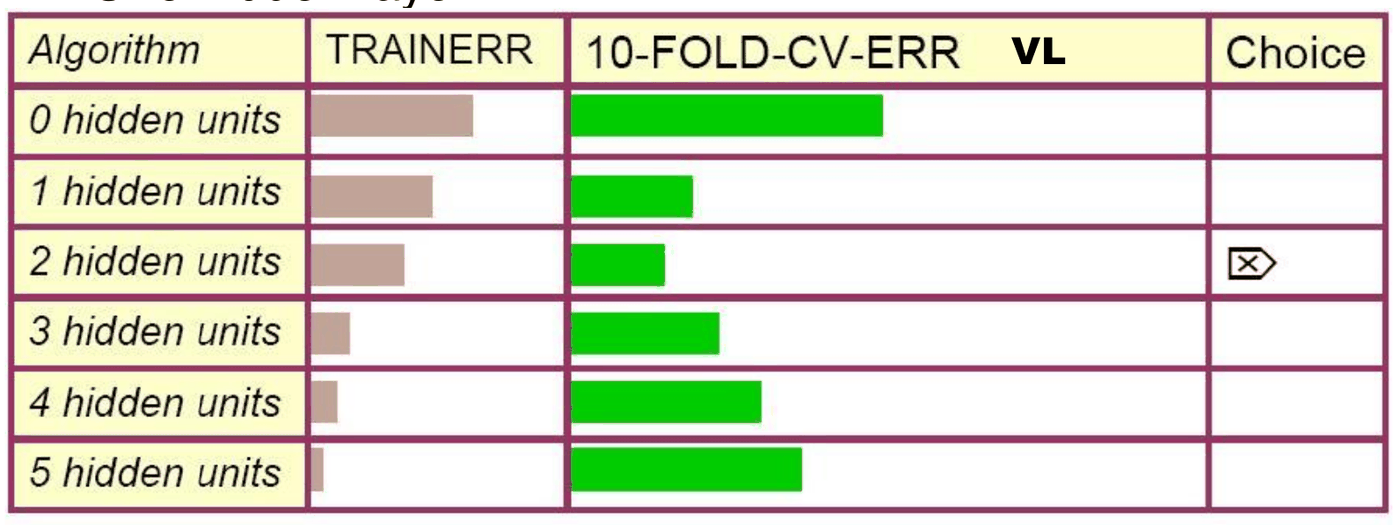
\includegraphics[width=0.86\linewidth,height=0.42\textheight,keepaspectratio]{images/11-val3_es-unita.png}
\caption{Choice of the number of hidden units of a network with one
hidden layer.}
\end{figure}

The training error always decreases with the number of units, but the
CV error has a minimum (here 2 units). In practice the search is done
over values such as 10, 20, 30\ldots{} (or with other steps).

\subsection{Example 3: K-NN}\label{esempio-3-k-nn}

\begin{figure}[htbp]
\centering
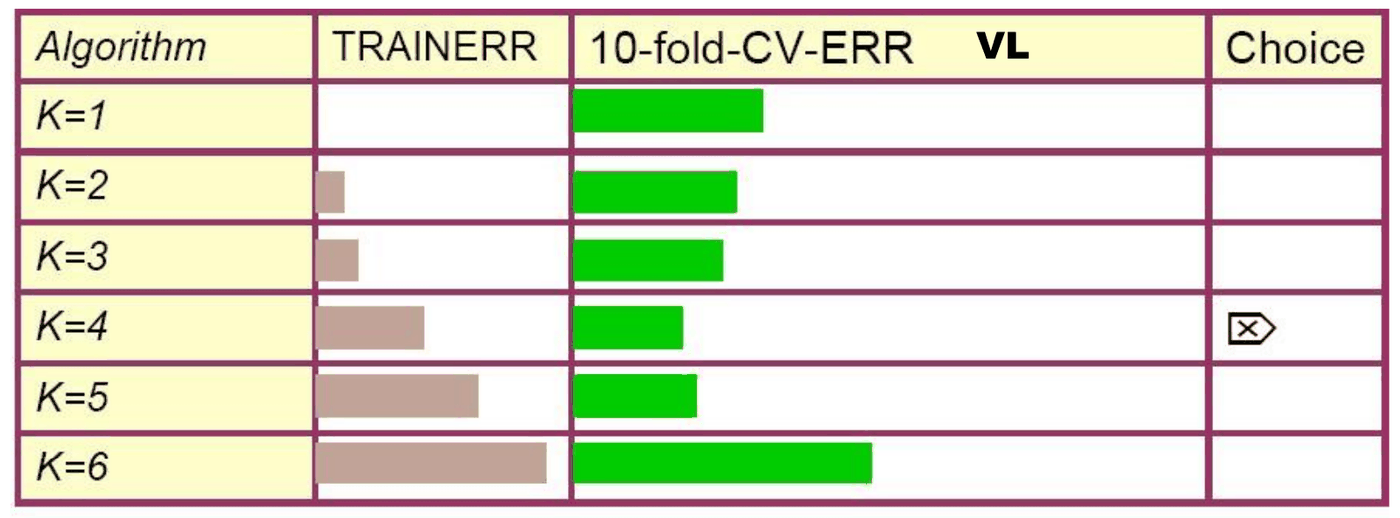
\includegraphics[width=0.86\linewidth,height=0.42\textheight,keepaspectratio]{images/11-val3_es-knn.png}
\caption{Choice of \(k\) for K-NN with leave-one-out CV.}
\end{figure}

Why \textbf{leave-one-out} for K-NN and 10-fold for networks? For
\textbf{computational} reasons: for K-NN (and other non-parametric
methods) LOOCV costs as much as a normal prediction (there is no model
to train). And why stop at \(K = 6\)? Only because things seemed to get
worse as \(K\) grew; and there is no guarantee that a local optimum of
\(K\) with respect to LOOCV is the global one (the relationship can be
very irregular). To explore many values one can use exponentially
growing values (\(K = 1, 2, 4, 8, 16, \dots\)) or a
\emph{hill-climbing} search starting from an initial value.

\section{Practical conclusions}\label{conclusioni-pratiche}

\begin{itemize}
\tightlist
\item
  \textbf{Simple hold-out} is widely used: sometimes the test set is
  already given separately or ``taken'' from previous applications. Be
  careful with few data and check the error rates on TR and VL.
\item
  \textbf{5- or 10-fold CV} is recommended as a good compromise
  (between bias and variance of the estimate) with respect to
  leave-one-out (Hastie et al.).
\end{itemize}

In the next lecture we go back to the \textbf{analytical} estimate of
the expected error, with Structural Risk Minimization and the
VC-dimension: it offers interesting insights for model selection and
comparison (where the \textbf{relative size} of the errors matters), as
an alternative to purely empirical evaluation.

\begin{boxquestion}{Possible exam questions}

\begin{itemize}
\tightlist
\item
  Why should training not be stopped after a fixed number of epochs?
\item
  How is early stopping handled with cross-validation and final
  retraining?
\item
  How to choose the final model with multiple random initialisations?
\item
  What is the sequential hyperparameter selection mistake?
\item
  Can cross-validation overfit? How can it be avoided?
\item
  Compare hold-out, K-fold and leave-one-out.
\end{itemize}

\end{boxquestion}
